\documentclass{beamer}

\usepackage{ifthen}
\usepackage{xparse}
\ExplSyntaxOn
\NewDocumentCommand{\getenv}{om}
{
  \sys_get_shell:nnN { kpsewhich ~ --var-value ~ #2 } { } \l_tmpa_tl
  \tl_trim_spaces:N \l_tmpa_tl
  \IfNoValueTF { #1 }
  {\tl_use:N \l_tmpa_tl}
  {\tl_set_eq:NN #1 \l_tmpa_tl}
}
\NewExpandableDocumentCommand{\ifstringsequalTF}{mmmm}
{
  \str_if_eq:eeTF { #1 } { #2 } { #3 } { #4 }
}
\ExplSyntaxOff

% Available mode: slides-only, notes-only, slides-notes-interlaced, slides-notes-dual (default)
\getenv[\BEAMERMODE]{BEAMERMODE}
\ifstringsequalTF{\BEAMERMODE}{slides-only}
{}
{
  \ifstringsequalTF{\BEAMERMODE}{notes-only}
  {\setbeameroption{show only notes}}
  {
    \ifstringsequalTF{\BEAMERMODE}{slides-notes-interlaced}
    {\setbeameroption{show notes}}
    {\setbeameroption{show notes on second screen=right}} % Default
  }
}

\usetheme{CambridgeUS}

\usepackage{svg}
\usepackage{amsmath}
\usepackage{listings}
\usepackage{ebproof}
\usepackage{hyperref}
\usepackage{transparent}
\usepackage{tikz}
\usetikzlibrary{positioning}
\usetikzlibrary{shadows.blur}
\usetikzlibrary{shapes.symbols}
\usetikzlibrary{tikzmark}
\usepackage[utf8]{inputenc}

%\usefonttheme[onlymath]{serif} % Use the same font as article

% Source: https://www.epfl.ch/about/overview/wp-content/uploads/2020/06/EPFL-brand-guidelines.pdf
\definecolor{epfl-rouge}{RGB}{255,0,0}
\definecolor{epfl-groseille}{RGB}{181,31,31}
\definecolor{epfl-leman}{RGB}{0,167,159}
\definecolor{epfl-canard}{RGB}{0,116,128}
\definecolor{epfl-taupe}{RGB}{65,61,58}
\definecolor{epfl-perle}{RGB}{200,199,199}


\setbeamercolor*{palette primary}{bg=epfl-taupe, fg=white}
\setbeamercolor*{palette secondary}{bg=epfl-perle, fg=black}
\setbeamercolor*{palette tertiary}{bg=epfl-groseille, fg=white}
%\setbeamercolor*{palette quaternary}{bg=blue, fg=green}

\setbeamercolor{itemize item}{fg=epfl-groseille}
\setbeamercolor{itemize subitem}{fg=epfl-leman}
\setbeamercolor{itemize subsubitem}{fg=epfl-taupe}

\setbeamercolor{titlelike}{bg=black!2}

\setbeamertemplate{itemize item}[circle]
\setbeamertemplate{itemize subitem}[square]
\setbeamertemplate{itemize subsubitem}[triangle]

\setbeamertemplate{section in toc}[sections numbered]
\setbeamertemplate{subsection in toc}[subsections numbered] % (unused)

% Section slide
% Does not rely on \AtBeginSection
\newcommand{\makesection}[1]{
  \begin{frame}
  \vfill
  \centering
  \begin{beamercolorbox}[sep=8pt,center,shadow=true,rounded=true]{title}
    \usebeamerfont{title}\insertsectionnumber. \insertsectionhead\par%
  \end{beamercolorbox}
  \vfill
  \note{#1}
  \end{frame}
}

% Adapted from https://tex.stackexchange.com/a/4199
\makeatletter
\newcommand*\idstyle{%
  \expandafter\id@style\the\lst@token\relax
}
\def\id@style#1#2\relax{%
  \ifcat#1\relax\else
    \ifnum`#1=\uccode`#1%
      \color{epfl-canard}
    \fi
  \fi
}
\makeatother

\lstset{
  language=Scala,
  showstringspaces=false,
  %xleftmargin=0.75cm,
  basicstyle=\ttfamily,
  captionpos=b,
  commentstyle=\color{epfl-perle}\textit,
  stringstyle=\color{epfl-groseille},
  keywordstyle=\color{epfl-rouge},
  identifierstyle=\color{epfl-taupe}\idstyle,%\color{epfl-leman},
  escapeinside={(@}{@)},
}

\newcommand{\lstid}[1]{{\color{epfl-taupe}{#1}}}

\beamertemplatenavigationsymbolsempty % Remove navigation bar
\setbeamercovered{transparent} % Make future content transparent

\newcommand{\code}{\texttt}

% Footnote with symbols rather than numbers
\makeatother
\renewcommand{\thefootnote}{\ifcase\value{footnote}\or{*}\or{**}\or{***}\fi}
\makeatletter
% Reset footnote numbering on each frame
\AtBeginEnvironment{frame}{\setcounter{footnote}{0}}

\let\oldemptyset\emptyset
\let\emptyset\varnothing

% Contents

\title[Master Thesis]{A front-end for the LISA proof assistant}
\subtitle{Master Thesis}
\author{Florian Cassayre}
\date{June 2022}

\institute[EPFL]{École polytechnique fédérale de Lausanne \\ School of Computer Science \\ \vspace{0.5cm}\includesvg[width=4cm]{figures/epfl-logo}}
\date{2022-07-21}
\day=21\relax
\month=07\relax
\year=2022\relax

\begin{document}

\begin{center}
{\LARGE \textbf{École Polytechnique Fédérale de Lausanne}} \\
\vspace{0.2cm}
{\Large {School of Computer Science}} \\
\vspace{1cm}

\includesvg[width=4cm]{figures/epfl-logo} \\
\vspace{0.8cm}

{\Large {Master Thesis}} \\
\vspace{1cm}

{\LARGE \textbf{A front-end for LISA}} \\
\vspace{1cm}

\end{center}

\begin{multicols}{2}
\hbadness=10000 % Suppress warning
\hfuzz=10pt %

\noindent{\large{Supervisor:}} \\
\large{\textbf{Prof. Viktor Kunčak}} \\
\vspace{0.1cm}

\noindent{\large{Assistant:}} \\
\large{\textbf{Simon Guilloud}} \\
\vspace{0.1cm}

\noindent{\large{External expert:}} \\
\large{\textbf{Prof. Jasmin Blanchette}} \\
\vspace{0.1cm}
\columnbreak

\noindent{\large{Candidate:}} \\
\large{\textbf{Florian Cassayre}} \\
\end{multicols}

\vspace{2cm}

\begin{center}
  \large{\textbf{June 2022}}
  %\large{\textbf{21.02.2022 until 24.06.2022}}
\end{center}

\begin{frame}{Outline}

\setcounter{tocdepth}{1}
\tableofcontents

\notes{
\begin{itemize}
\item This is the agenda of the presentation. I am not going to cover all the details of my work, but rather give a high-level overview that will hopefully be comprehensive enough for those that are not necessarily familiar with the field of study.
\item I will start by introducing you to LISA, which the core tool that my project builds onto.
\item Then I will describe the possibilities offered by my framework to write proofs.
\item I will discuss in more details about a particular matching procedure for sequent calculus that I designed for the framework.
\item Finally I will showcase the language features of the framework.
\end{itemize}
}
{
\begin{itemize}
\item agenda, coverage
\item start introducing LISA
\item then, possibilities write proofs
\item more details matching
\item showcase language features
\end{itemize}
}

\end{frame}

\section{Introduction}
\label{sec:introduction}

A proof assistant is a piece of software that can assist a human user in writing a particular type of proofs, one that can be verified by a machine. Proofs following this format are desirable because it suffices to show that the verification procedure is sound to automatically and irrefutably judge any of them. Computer-assisted theorem proving can also leverage the computational capabilities offered by machines, one of the most famous example being the proof of the \textit{four-color conjecture} \cite{Appel1989}. However, the greatest strength of proof assistants might also be their greatest weakness: they are often complex systems, whose correctness is difficult to demonstrate and therefore are prone to bugs in their implementation. They also suffer from a lack of understandability, both in terms of the underlying theories used and of the proofs produced, which results in a low adoption rate by mathematicians \cite{Ayers2021}.

In this thesis we describe the design process of a front-end for the modern proof assistant LISA. Our main focus is to preserve the same soundness standards as the existing framework while making it more expressive and interactive. The supporting source code for this project is published at the following address:
\begin{center}
\href{http://github.com/FlorianCassayre/master-project}{\textbf{github.com/FlorianCassayre/master-project}}\footnote{The current release is identified by commit number: \code{30b0c340e94c6e981d3115c554ab9bc97f8b8971}}
\end{center}

\subsection{LISA}

LISA\footnote{\textbf{L}ISA \textbf{I}s \textbf{S}ets \textbf{A}utomated} is an ongoing project conducted at the Lab for Automated Reasoning and Analysis (LARA), EPFL. It is a library built on top of sequent calculus and set theory that enables the formalization of mathematical proofs \cite{Guilloud2022-2}.

\begin{figure}[H]
  $$
  \begin{prooftree}
  \hypo{}
  \infer1[Hypo.]{{?a} \vdash {?a}, {?b}}
  \infer1[Left $\neg$]{\neg{?a}, {?a} \vdash {?b}}
  \hypo{}
  \infer1[Hypo.]{{?a}, {?b} \vdash {?b}}
  \infer2[Left $\lor$]{\neg{?a} \lor {?b}, {?a} \vdash {?b}}
  \infer1[Right $\Rightarrow$]{\neg{?a} \lor {?b} \vdash {?a} \Rightarrow {?b}}
  \infer1[Right $\Rightarrow$]{\vdash \neg{?a} \lor {?b} \Rightarrow {?a} \Rightarrow {?b}}
  %
  \hypo{}
  \infer1[Hypo.]{{?a} \vdash {?a}, {?b}}
  \infer1[Right $\neg$]{\vdash \neg{?a}, {?a}, {?b}}
  \hypo{}
  \infer1[Hypo.]{{?b} \vdash \neg{?a}, {?b}}
  \infer2[Left $\Rightarrow$]{{?a} \Rightarrow {?b} \vdash \neg{?a}, {?b}}
  \infer1[Right $\lor$]{{?a} \Rightarrow {?b} \vdash \neg{?a} \lor {?b}}
  \infer1[Right $\Rightarrow$]{\vdash ({?a} \Rightarrow {?b}) \Rightarrow \neg{?a} \lor {?b}}
  %
  \infer2[Right $\Leftrightarrow$]{\vdash \neg{?a} \lor {?b} \Leftrightarrow {?a} \Rightarrow {?b}}
  \end{prooftree}
  $$
  \caption[Proof tree (1)]{An example of a proof in sequent calculus. This proof demonstrates the tautology $\neg{?a}\lor{?b}\Leftrightarrow{?a}\Rightarrow{?b}$. The question mark indicates a schema, namely a variable that can later be instantiated. The inference rule used at every step is indicated on the right.}
  \label{fig:simple-lisa-proof-graph}
\end{figure}

\begin{figure}[H]
  \centering
  \small
$\begin{array}{r@{\hskip 0.1cm}rll@{\hskip 1cm}r}
0   &  & \text{Hypo.}~                       & {?a} \vdash {?a}; {?b}                                          & [{?a}] \\
1   &  & \text{Subproof}~0                   & \vdash \neg{?a} \lor {?b} \Rightarrow {?a} \Rightarrow {?b}     & \\
 &  -1 & \text{Import}~                      & {?a} \vdash {?a}; {?b}                                          & \\
 &   0 & \text{Left}~{\neg}~{-1}             & \neg{?a}; {?a} \vdash {?b}                                      & [{?a}] \\
 &   1 & \text{Hypo.}~                       & {?a}; {?b} \vdash {?b}                                          & [{?b}] \\
 &   2 & \text{Left}~{\lor}~0, 1             & \neg{?a} \lor {?b}; {?a} \vdash {?b}                            & [\neg{?a}; {?b}] \\
 &   3 & \text{Right}~{\Rightarrow}~2        & \neg{?a} \lor {?b} \vdash {?a} \Rightarrow {?b}                 & [{?a}; {?b}] \\
 &   4 & \text{Right}~{\Rightarrow}~3        & \vdash \neg{?a} \lor {?b} \Rightarrow {?a} \Rightarrow {?b}     & [\neg{?a} \lor {?b}; {?a} \Rightarrow {?b}] \\
2   &  & \text{Subproof}~0                   & \vdash ({?a} \Rightarrow {?b}) \Rightarrow \neg{?a} \lor {?b}   & \\
 &  -1 & \text{Import}~                      & {?a} \vdash {?a}; {?b}                                          & \\
 &   0 & \text{Right}~{\neg}~{-1}            & \vdash \neg{?a}; {?a}; {?b}                                     & [{?a}] \\
 &   1 & \text{Hypo.}~                       & {?b} \vdash \neg{?a}; {?b}                                      & [{?b}] \\
 &   2 & \text{Left}~{\Rightarrow}~0, 1      & {?a} \Rightarrow {?b} \vdash \neg{?a}; {?b}                     & [{?a}; {?b}] \\
 &   3 & \text{Right}~{\lor}~2               & {?a} \Rightarrow {?b} \vdash \neg{?a} \lor {?b}                 & [\neg{?a}; {?b}] \\
 &   4 & \text{Right}~{\Rightarrow}~3        & \vdash ({?a} \Rightarrow {?b}) \Rightarrow \neg{?a} \lor {?b}   & [{?a} \Rightarrow {?b}; \neg{?a} \lor {?b}] \\
3   &  & \text{Right}~{\Leftrightarrow}~1, 2 & \vdash \neg{?a} \lor {?b} \Leftrightarrow {?a} \Rightarrow {?b} & [\neg{?a} \lor {?b}; {?a} \Rightarrow {?b}]
\end{array}$
\normalsize

  \caption[Proof in LISA]{A representation of the proof of \autoref{fig:simple-lisa-proof-graph} in LISA. Each step is assigned an index, and import are represented with negative indices. Scoping within the proof is possible and determined by the indentation level: subproofs are indented further down. The second column states what rule is used, along with the premises it uses. The third column is the conclusion of that step. The last column contains parameters to disambiguate the application of the rule.}
  \label{fig:simple-lisa-proof}
\end{figure}

A proof in this system is a directed acyclic graph of proof steps. Each such step corresponds to the application of an inference rule, and is characterized by its conclusion expressed as a sequent, and some premises. A sequent is a pair of sets of formulas, noted $\phi_1, \phi_2, ..., \phi_n \vdash \psi_1, \psi_2, ..., \psi_m$ or $\Gamma \vdash \Delta$, and can be interpreted in conventional logic as a conjunction of premises implying a disjunction of conclusions. That said, the actual semantic is controlled by the inference rules provided by the system. Proofs can optionally have ``imports'': sequents that are used as premises but do not come from any step. Proofs may also be nested for organization purposes. Figures \ref{fig:simple-lisa-proof-graph} and \ref{fig:simple-lisa-proof} showcase a formal proof in LISA. Notice that a directed acyclic graph can always be represented in a linear fashion, but not necessarily as a tree (unless we duplicate forward edges).

Currently LISA only exists as a Scala library, therefore the proofs are described using Scala code. For further technical details about LISA, we refer the reader to the official manual \cite{Guilloud2022-2}.

\section{Proofs}

\makesection{
\begin{itemize}
\item This is precisely what I will present in this second part. Namely how the proofs are would be written in the front-end layer.
\end{itemize}
}

\subsection{Patterns}

\newcommand{\Cphi}{{\color{epfl-rouge}\phi}}
\newcommand{\Ca}{{\color{epfl-rouge!70}{?a}}}
\newcommand{\Cpsi}{{\color{epfl-leman}\psi}}
\newcommand{\Cb}{{\color{epfl-leman!70}{?b}}}
\newcommand{\Cx}{{\color{epfl-canard}x}}
\newcommand{\Cp}{{\color{epfl-rouge!70}{?p}}}
\newcommand{\Ct}{{\color{gray}{?t}}}

\begin{frame}{Patterns}
\framesubtitle{Generalizing inference rules}

\begin{align*}
\text{LISA rule:} \qquad\qquad &\hphantom{\longrightarrow} \qquad\quad \text{Corresponding pattern:} \\
\begin{prooftree}
\hypo{\vphantom{\Gamma}}
\infer1{\Gamma, \Cphi \vdash \Cphi, \Delta}
\end{prooftree}
\qquad
&\longrightarrow
\qquad
\begin{prooftree}
\hypo{\vphantom{\Gamma}}
\infer1{..., \Ca \vdash \Ca, ...}
\end{prooftree}
\tag{Hypothesis}
\\[0.5cm] %
\begin{prooftree}
\hypo{\Gamma, \Cphi \vdash \Delta}
\hypo{\Sigma, \Cpsi \vdash \Pi}
\infer2{\Gamma, \Sigma, \Cphi \lor \Cpsi \vdash \Delta, \Pi}
\end{prooftree}
\qquad
&\longrightarrow
\qquad
\begin{prooftree}
\hypo{..., \Ca \vdash ...}
\hypo{..., \Cb \vdash ...}
\infer2{..., \Ca \lor \Cb \vdash ...}
\end{prooftree}
\tag{Left $\lor$}
\\[0.5cm] %
\begin{prooftree}
\hypo{\Gamma \vdash \exists \Cx. \Cphi, \Delta}
\infer1{\Gamma \vdash \Cphi [\Cx \mapsto \Ct], \Delta}
\end{prooftree}
\qquad
&\longrightarrow
\qquad
\begin{prooftree}
\hypo{... \vdash \exists \Cx. \Cp(\Cx), ...}
\infer1{... \vdash \Cp(\Ct), ...}
\end{prooftree}
\tag{Right $\exists$}
\\[0.5cm] %
\begin{prooftree}
\hypo{\Gamma \vdash \Delta}
\infer1{(\Gamma \vdash \Delta) [{?p} \mapsto \phi(\Psi)]}
\end{prooftree}
\qquad
&\longrightarrow
\qquad
?
\tag{Inst. Pred.}
\end{align*}

\note{
\begin{itemize}
\item The first contribution I am going to present is patterns. Patterns are a generalized representation of rules.
\item On the left side is a LISA rule and on the right side is the corresponding pattern. The common symbols are highlighted in the same color for clarity. Notice that we represent the static formulas as schemas in our patterns. Therefore patterns do not need any extension to first order logic. I will come back to the actual meaning of the ellipsis.
\item Unfortunately not all rules have a representation in our system, for examples rules that act on all the formulas of a sequent such as the predicate instantiation rule.
\end{itemize}
}

\end{frame}

\begin{frame}{Patterns}
\framesubtitle{Motivations}

\begin{itemize}
\item Automatic inference of parameters
\item Forward and backward reasoning
\item Encapsulate multiple rules into a single pattern
\end{itemize}

\note{
\begin{itemize}
\item One may wonder the motivation behind the introduction of these rules. There are in fact several reasons.
\item The first one is that by having unified the representation of the rules, it allows us to design algorithms that work on all rules by extension. One such algorithm is an inference procedure that can automatically deduce the value of the schemas in the pattern without having the need for the user to specify them.
\item Another reason is that they can be used forward and backward without additional logic. We will see later what we mean by that.
\item A chain of rules can also be represented by a single pattern.
\end{itemize}
}

\end{frame}

\begin{frame}{Patterns}
\framesubtitle{Combining multiple rules together}

Entire branches can be represented by a single pattern:

\scriptsize
\begin{align*}
\begin{prooftree}
\hypo{\Gamma \vdash \Cphi \lor \Cpsi, \Delta}
\hypo{\vphantom{\Gamma}}
\infer1[Hypothesis]{\Cphi \vdash \Cphi}
\hypo{\vphantom{\Gamma}}
\infer1[Hypothesis]{\Cpsi \vdash \Cpsi}
\infer2[Left $\lor$]{\Cphi \lor \Cpsi \vdash \Cphi, \Cpsi}
\infer2[Cut]{\Gamma \vdash \Cphi, \Cpsi, \Delta}
\end{prooftree}
&\longrightarrow
\quad
\begin{prooftree}
\hypo{... \vdash \Ca \lor \Cb, ...}
\infer1[Elim. R. $\lor$]{... \vdash \Ca, \Cb, ...}
\end{prooftree}
\end{align*}
\normalsize

\note{
\begin{itemize}
\item This representation makes is possible to factor out multiple branches into a single pattern application.
\item For example, LISA only provides what we call introduction rules (rules where the bottom sequent introduces a new symbol). However it turns out there are instances where it is desirable to go the other way around. This is possible since most rules are conservative, meaning that the conclusion is not weaker that the hypotheses (and vice versa). We call these rules elimination, and the one presented here is such an example.
\end{itemize}
}

\end{frame}

% Direction

\begin{frame}[fragile]
\frametitle{Proof direction}
\framesubtitle{Forward and backward styles}

\begin{itemize}
\item Forward (top-down): combining true statements together
\item Backard (bottom-up): begin with the conclusion and close the branches
\end{itemize}



\note{
\begin{itemize}
\item .
\end{itemize}
}

\end{frame}

\begin{frame}[fragile]
\frametitle{Mixed styles}

\centering

{\scriptsize\begin{lstlisting}
(@\onslide<1,6>@)val theorem: Theorem = ProofMode(sequent"|- ({} in {}) => ?a")
  .pipe { p =>
    import p.* (@\onslide<1,2,6>@)
    apply(introRImp) (@\onslide<1,3,6>@)
    apply(elimRNot) (@\onslide<1,6>@)
    (@\onslide<1,5,6>@)apply(justificationInst(
      (@\onslide<1,4,5,6>@)elimRForall(AssignedFunction(t, s))(axiomEmpty)(@\onslide<1,5,6>@)
    ))(@\onslide<1,6>@)
    asTheorem()
  }
\end{lstlisting}}

\onslide<1->

\newcommand{\rw}[1]{\rewrite{#1\box\treebox}}
\newcommand{\mkinvisible}[0]{\transparent{0.15}}
\newcommand{\mkvisible}[0]{\transparent{1}}

{\tiny\begin{prooftree}
\hypo{\vdash \forall x. \neg(x \in \varnothing)}
\rw{\only<4>{\mkinvisible}}
\hypo{}
\infer1[$\text{Hypo.}$]{\neg({?s} \in \varnothing) \vdash \neg({?s} \in \varnothing)}
\infer1[$\text{Left}~{\forall}$]{\forall x. \neg(x \in \varnothing) \vdash \neg({?s} \in \varnothing)}
\infer2[$\text{Cut}$]{\vdash \neg({?s} \in \varnothing)}
\rw{\only<4>{\mkvisible}}
\infer1[$\text{?Fun. Instantiation}$]{\vdash \neg(\varnothing \in \varnothing)}
\infer1[$\text{Weakening}$]{\vdash \neg(\varnothing \in \varnothing); {?a}}
\rw{\only<3>{\mkinvisible}}
\rw{\only<5>{\mkvisible}}
\hypo{}
\infer1[$\text{Hypo.}$]{\varnothing \in \varnothing \vdash \varnothing \in \varnothing}
\infer1[$\text{Left}~{\neg}$]{\neg(\varnothing \in \varnothing); \varnothing \in \varnothing \vdash}
\infer2[$\text{Cut}$]{\varnothing \in \varnothing \vdash {?a}}
\rw{\only<2>{\mkinvisible}\only<3>{\mkvisible}}
\infer1[$\text{Right}~{\Rightarrow}$]{\vdash (\varnothing \in \varnothing) \Rightarrow {?a}}
\rw{\only<3-5>{\mkinvisible}}
\end{prooftree}}

\end{frame}

\section{Matching}

\section{Language features}

\makesection{
\notes{
\begin{itemize}
\item In this fourth section, I will be discussing about the features related to the domain specific language, as well as the interoperability possibilities.
\end{itemize}
}
{
\begin{itemize}
\item fourth section: features DSL, possibilities for interoperability
\end{itemize}
}
}

\subsection{Type safe DSL}

\begin{frame}[fragile]
\frametitle{Domain specific language}
\framesubtitle{Precise typing of labels}

\onslide<1>

\begin{lstlisting}
val a = SchematicPredicateLabel[0]("a")

a /\ (!a ==> a): Formula (@\onslide<2-3>@)

val t = SchematicFunctionLabel[0]("t") (@\onslide<2>@)
val p = SchematicPredicateLabel[1]("p")

p(t): Formula
p(t, t): Formula // error (@\onslide<3>@)

val f = LambdaFunction[1](t1 => t1)
f(t): Term
\end{lstlisting}

\only<1>{
\notes{
\begin{itemize}
\item The framework I designed also defines its own domain specific language, that provides additional compile-time safety guarantees to that of LISA's making it safer at usage.
\item For instance, the labels have their arity encoded as a singleton type. A singleton type has the special property that it can be translated into a value at compilation time: here "0" is a literal type, which is by extension a singleton type.
\item The motivation for that is to enforce the correct number of arguments. "a" does not expect any argument here and so its usage in this context is legal.
\end{itemize}
}
{
\begin{itemize}
\item framework DSL, typesafety
\item labels arity encoded singleton type; singleton type $\rightarrow$ value
\item literal type (e.g. "0") are singleton
\item allows to enforce correct number of args
\item here "a" does not take any args
\end{itemize}
}
}

\only<2>{
\notes{
\begin{itemize}
\item This is illustrated in that second example. "p" expects one argument. Passing more than one argument will trigger a type error.
\end{itemize}
}
{
\begin{itemize}
\item illustrated here, "p" expects 1
\item error
\end{itemize}
}
}

\only<3>{
\notes{
\begin{itemize}
\item We also provide convenient constructors for lambda terms. They are represented as values at runtime, rather than Scala functions. They are used in substitutions.
\end{itemize}
}
{
\begin{itemize}
\item also constructors for lambdas
\item represented as value, instantiation = substitution
\end{itemize}
}
}

\end{frame}

\begin{frame}[fragile]
\frametitle{String interpolation}
\framesubtitle{Multi-stage programming (macros)}

\onslide<1-2>

\begin{lstlisting}
val f1: Formula = formula"?a /\ (!?a => ?a)" (@\onslide<2>@)

val p = SchematicPredicateLabel[1]("p")

sequent"|- (@\lstid{\$f1}@); (@\lstid{\$p}@)(?t)" (@\onslide<3>@)

val x = VariableLabel("x")

formula"forall (@\lstid{\$x}@). ?p((@\lstid{\$x}@))"
\end{lstlisting}

\only<1>{
\notes{
\begin{itemize}
\item The framework also defines a language for sequents and formulas, which can be parsed and printed. Without entering into the details I will present an interesting language feature that is used; that is string interpolation.
\item In Scala string interpolation is a syntactic sugar that allows us to translate a string into something else. The particularity is that the string can contain Scala expressions as well.
\item The "formula" interpolator allows the seamless conversion of a string to a formula. The parsing is done at compilation time making it safe at usage.
\end{itemize}
}
{
\begin{itemize}
\item language for sequents, parsed/printed
\item interesting language feature: string interpolation
\item syntactic sugar to translate a string
\item particularity: expressions in between
\item "formula" interpolator
\item compilation time: typesafe, clear errors, no overhead
\end{itemize}
}
}

\only<2>{
\notes{
\begin{itemize}
\item This second examples shows how expressions can be inserted into the interpolator.
\item For instance, a formula "f1" or a pattern "p". Again, the types and arities are checked at compilation time for correctness.
\end{itemize}
}
{
\begin{itemize}
\item how expressions can be inserted
\item types and arities checked for correctness
\end{itemize}
}
}

\only<3>{
\notes{
\begin{itemize}
\item Bound variables are also supported; the binding relation is detected thanks to singleton types.
\end{itemize}
}
{
\begin{itemize}
\item bound variables, singleton types
\end{itemize}
}
}

\end{frame}

\subsection{Interoperability}

\begin{frame}{Interoperability}

\begin{itemize}
\item Proof compression routines
\item Human-readable SerDes of proofs
\item Export proofs and notations to {\rmfamily\LaTeX}
\end{itemize}

\notes{
\begin{itemize}
\item Before I conclude, I want to shed light on the interoperability features offered by the framework.
\item As we have seen, it is capable of converting a high-level proof into a LISA proof. Such process can sometimes create needless steps. To address that I implemented a set of procedures that can simplify a proof in length, depth and computational complexity.
\item Such proofs can then be serialized into a human-readable language that I designed which can later be efficiently deserialized.
\item Finally these proofs can also be typesetted thanks to a LaTeX printer.
\end{itemize}
}
{
\begin{itemize}
\item before conclude, other features
\item capable producing proofs, however proofs longer needed; procedures to simplify
\item human-readable serializer, representation can be deserialized back
\item proof/notations typesetted to latex
\end{itemize}
}

\end{frame}

\section{Conclusion}

\makesection{
\notes{
\begin{itemize}
\item I will now recap the contributions of my framework.
\end{itemize}
}
{
\begin{itemize}
\item recap contributions
\end{itemize}
}
}

\subsection{Contributions}

\begin{frame}{Conclusion}

\begin{itemize}
\item Less involvement is required from the user
\item Versatile matching procedure
\item Proof generation
\item Rich language
\end{itemize}

\notes{
\begin{itemize}
\item Firstly, the framework provides a more expressive and dynamic way of writing proofs.
\item This is partly thanks to the proposed matching procedure which has inference capabilities, and can be applied to different use cases.
\item This framework ultimately generates LISA proofs that can be checked for correctness, exported or even imported.
\item Finally the rich and expressive languages simplifies the usage of this system.
\end{itemize}
}
{
\begin{itemize}
\item firstly, more expressive and dynamic
\item thanks to matching, inference, different use cases
\item only LISA trusted
\item rich language improves usability
\end{itemize}
}

\end{frame}

\subsection{References}

\begin{frame}{Material}

\centering

Source code: \href{https://github.com/FlorianCassayre/master-project}{\code{github.com/FlorianCassayre/master-project}}

\vspace{0.5cm}

\begin{tikzpicture}[image/.style={inner sep=0.3mm,outer sep=0,draw=none,shade,top color=gray,bottom color=gray,blur shadow={shadow blur steps=10}}]

\node[image] (e) [xshift=8cm, yshift=0cm] {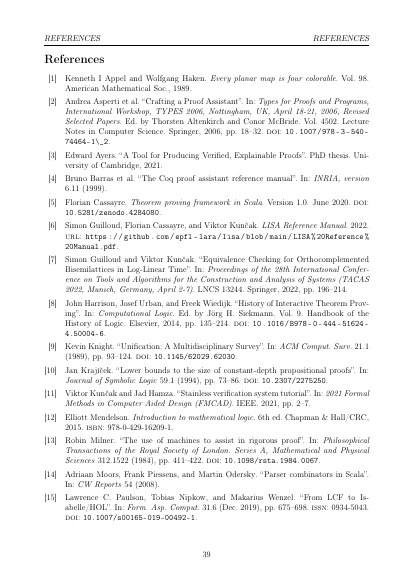
\includegraphics[height=4cm]{figures/thumbnail-39.png}};
\node[image] (d) [xshift=6cm, yshift=-0.5cm] {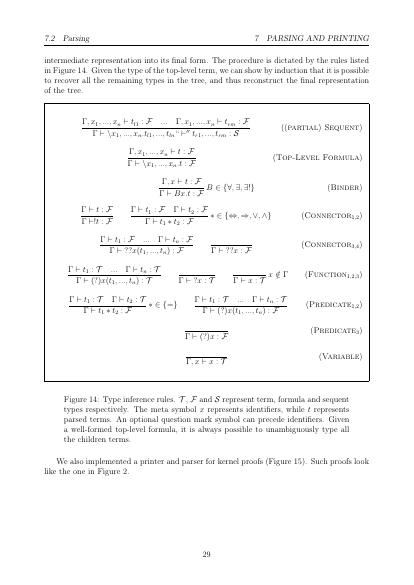
\includegraphics[height=4cm]{figures/thumbnail-29.png}};
\node[image] (c) [xshift=4cm, yshift=0cm] {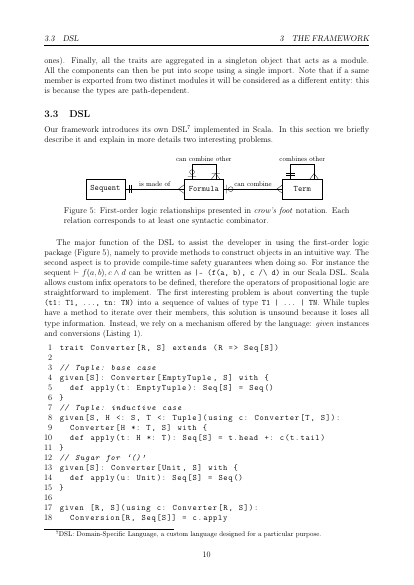
\includegraphics[height=4cm]{figures/thumbnail-10.png}};
\node[image] (b) [xshift=2cm, yshift=-0.5cm] {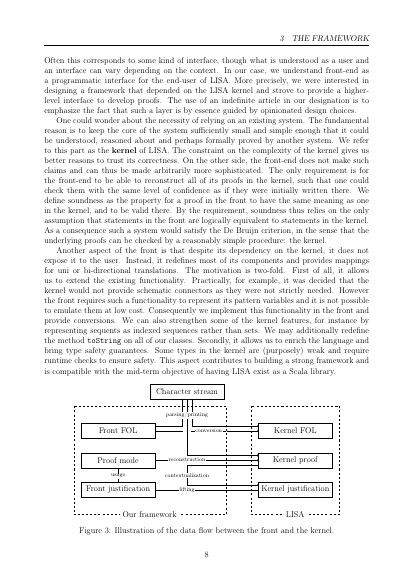
\includegraphics[height=4cm]{figures/thumbnail-08.png}};
\node[image] (a) {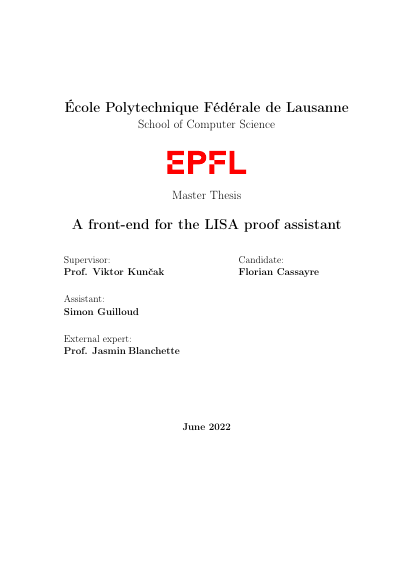
\includegraphics[height=4cm]{figures/thumbnail-01.png}};
\end{tikzpicture}

\vspace{0.5cm}

\href{https://zenodo.org/record/6645113}{\code{doi:10.5281/zenodo.6645113}}

\notes{
\begin{itemize}
\item The source code along with the thesis report is published on Zenodo.
\item Thank you very much for your attention. The first part of this presentation is over, I will now be taking and answering questions from the audience.
\end{itemize}
}
{
\begin{itemize}
\item source code and report on Zenodo
\item thanks; questions
\end{itemize}
}

\end{frame}


\end{document}
